\documentclass{beamer}
\usepackage{subfig}

\setbeamertemplate{footline}[frame number]
\title{Introduction to Machine Learning}
\author{Prof. Alessandro Lucantonio}
\institute{Aarhus University}
\date{7/10/2024}

\setbeamertemplate{navigation symbols}{}


\begin{document}
	
	\frame{\titlepage}
	
	\begin{frame}
		\frametitle{What is Machine Learning?}
		\begin{itemize}
			\item Arthur Samuel (1959). Machine learning is a ``Field of study that gives computers the ability to learn without being explicitly programmed”.
			\item Tom Mitchell (1998). ``A computer program is said to learn from experience \textit{E} with respect to some class of tasks \textit{T} and performance measure \textit{P}, if its performance at tasks in \textit{T}, as measured by \textit{P}, improves with experience \textit{E}”.
		\end{itemize}
		
	\end{frame}

	\begin{frame}		
		\frametitle{Some applications - Image recognition}
		\begin{figure}
			\centering
			\subfloat[\centering]{{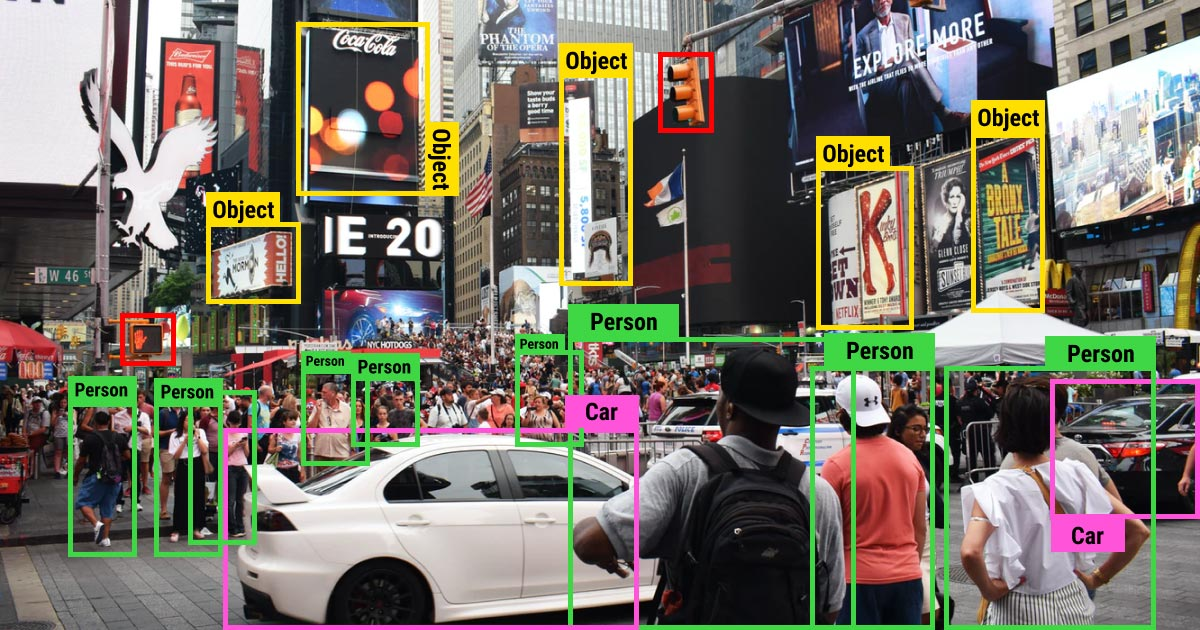
\includegraphics[scale=0.13]{images/image-recognition-1}}}
			\qquad
			\subfloat[\centering]{{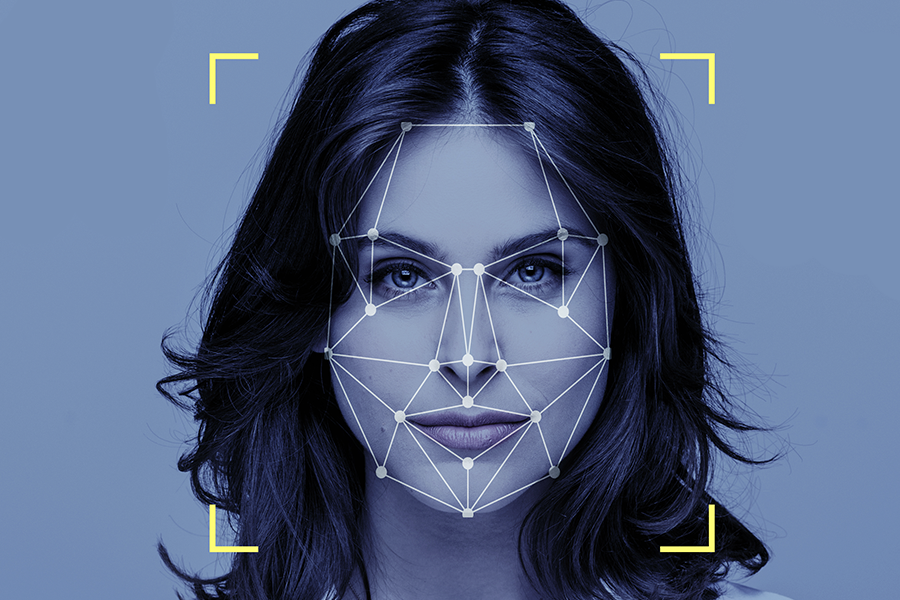
\includegraphics[scale=0.13]{images/image-recognition-2}}}
		\end{figure}
	Two examples of image recognition:
	
	(a) Labelling different entities in a given image.
	
	(b) Face recognition.
	\end{frame}

	\begin{frame}
	\frametitle{Some applications - Self-driving cars}
	\begin{figure}
		\centering
		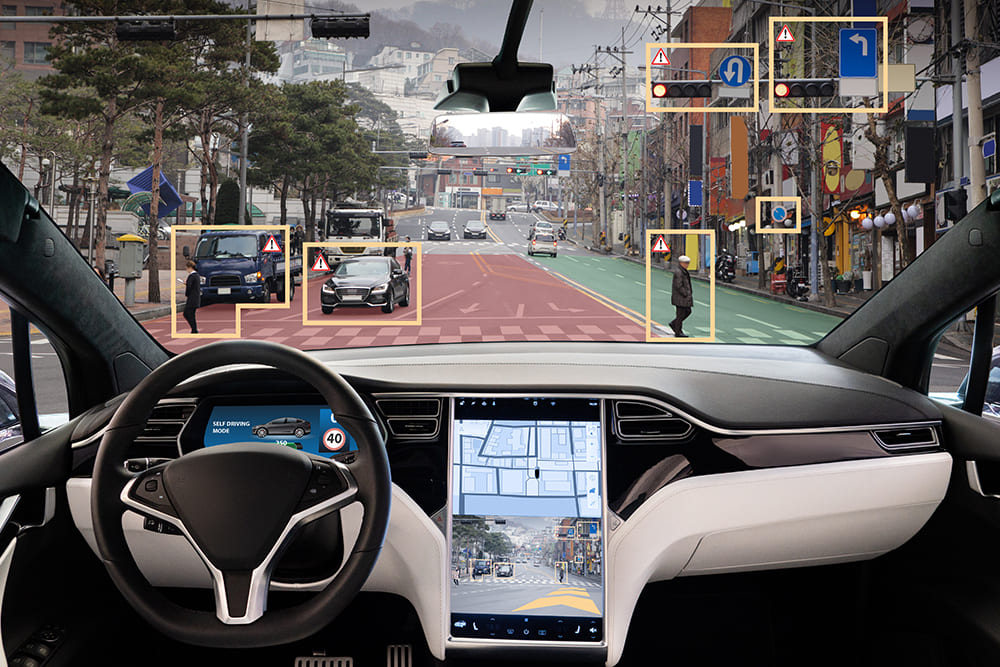
\includegraphics[scale=0.3]{images/self-driving-1}
	\end{figure}
	
\end{frame}

	\begin{frame}
		\frametitle{Some applications - Speech and voice recognition}
		\textit{Speech recognition} (or transcription) involves recording a speech using a recording device. The audio is then converted into a set of words stored digitally within the device or program. Instead, the purpose of \textit{voice recognition} is to identify the person who is speaking.
		\begin{figure}
			\centering
			\subfloat[\centering]{{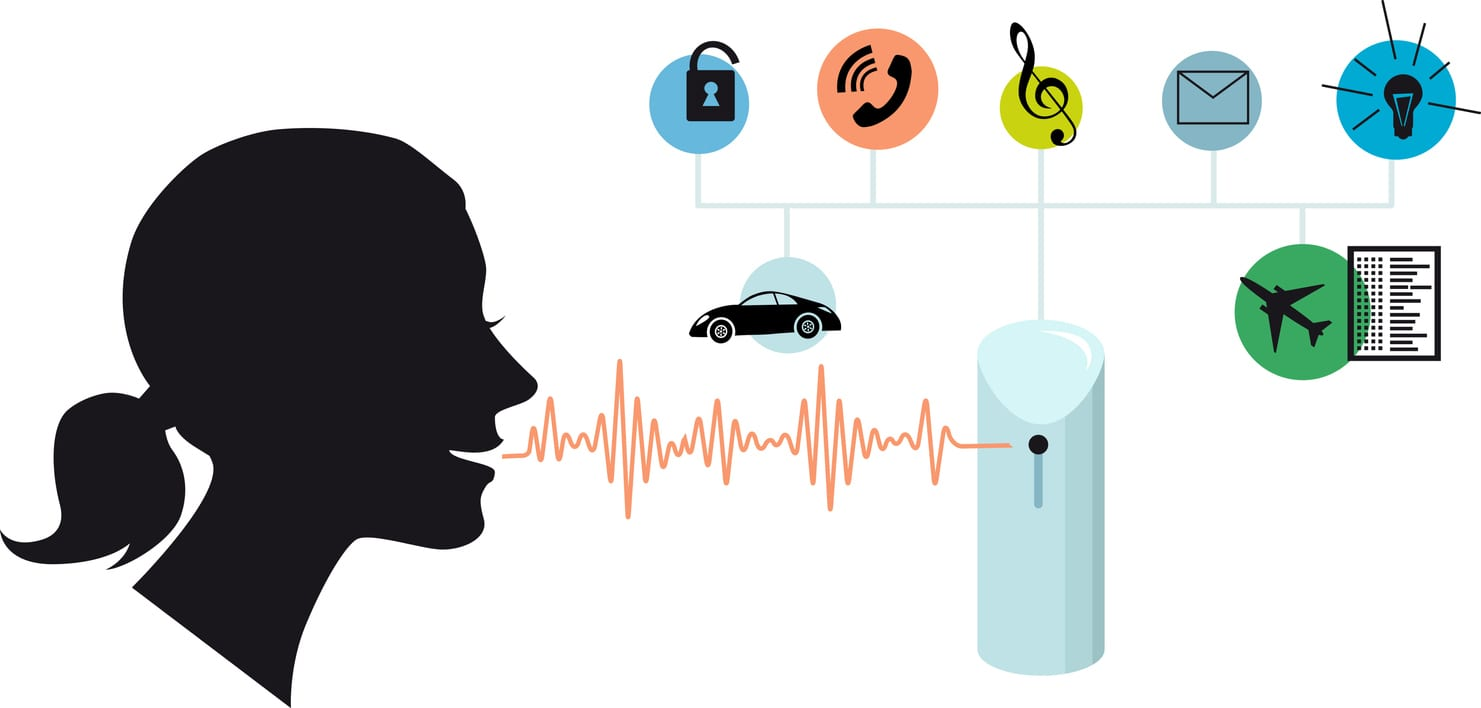
\includegraphics[scale=0.13]{images/speech-recognition-1}}}
			\qquad
			\subfloat[\centering]{{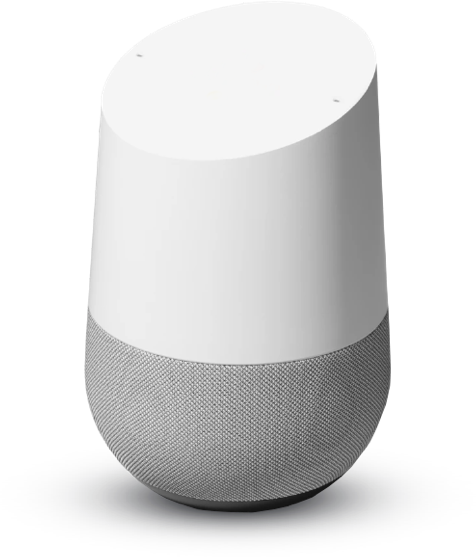
\includegraphics[scale=0.13]{images/speech-recognition-2}}}
		\end{figure}
	(c) A general idea of speech recognition. 
	
	(d) Google’s voice assistant provide individualized responses (e.g. calendar updates or reminders) only to the users who trained the assistant to recognize their voices.
	
	\end{frame}

	\begin{frame}
		\frametitle{Some applications - Email spam filtering}
		Task: determine if a given email is spam or not.
		\begin{figure}
			\centering
			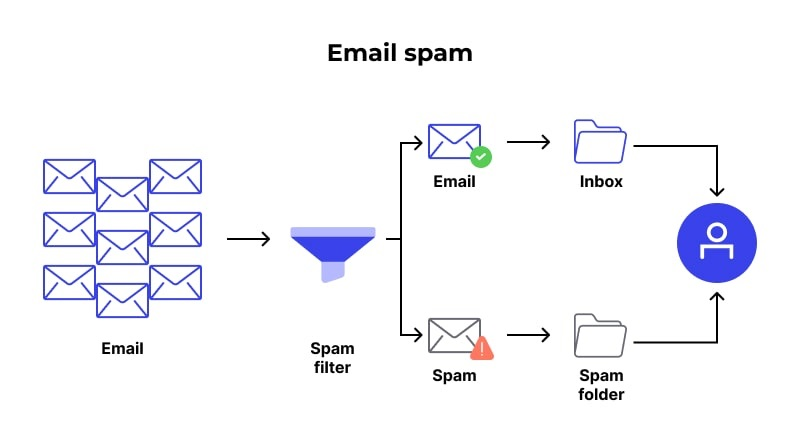
\includegraphics[scale=0.5]{images/spam-filtering-1}
		\end{figure}
	\end{frame}

	\begin{frame}
		\frametitle{Some applications - Learning how to play games}
		\begin{figure}
			\centering
			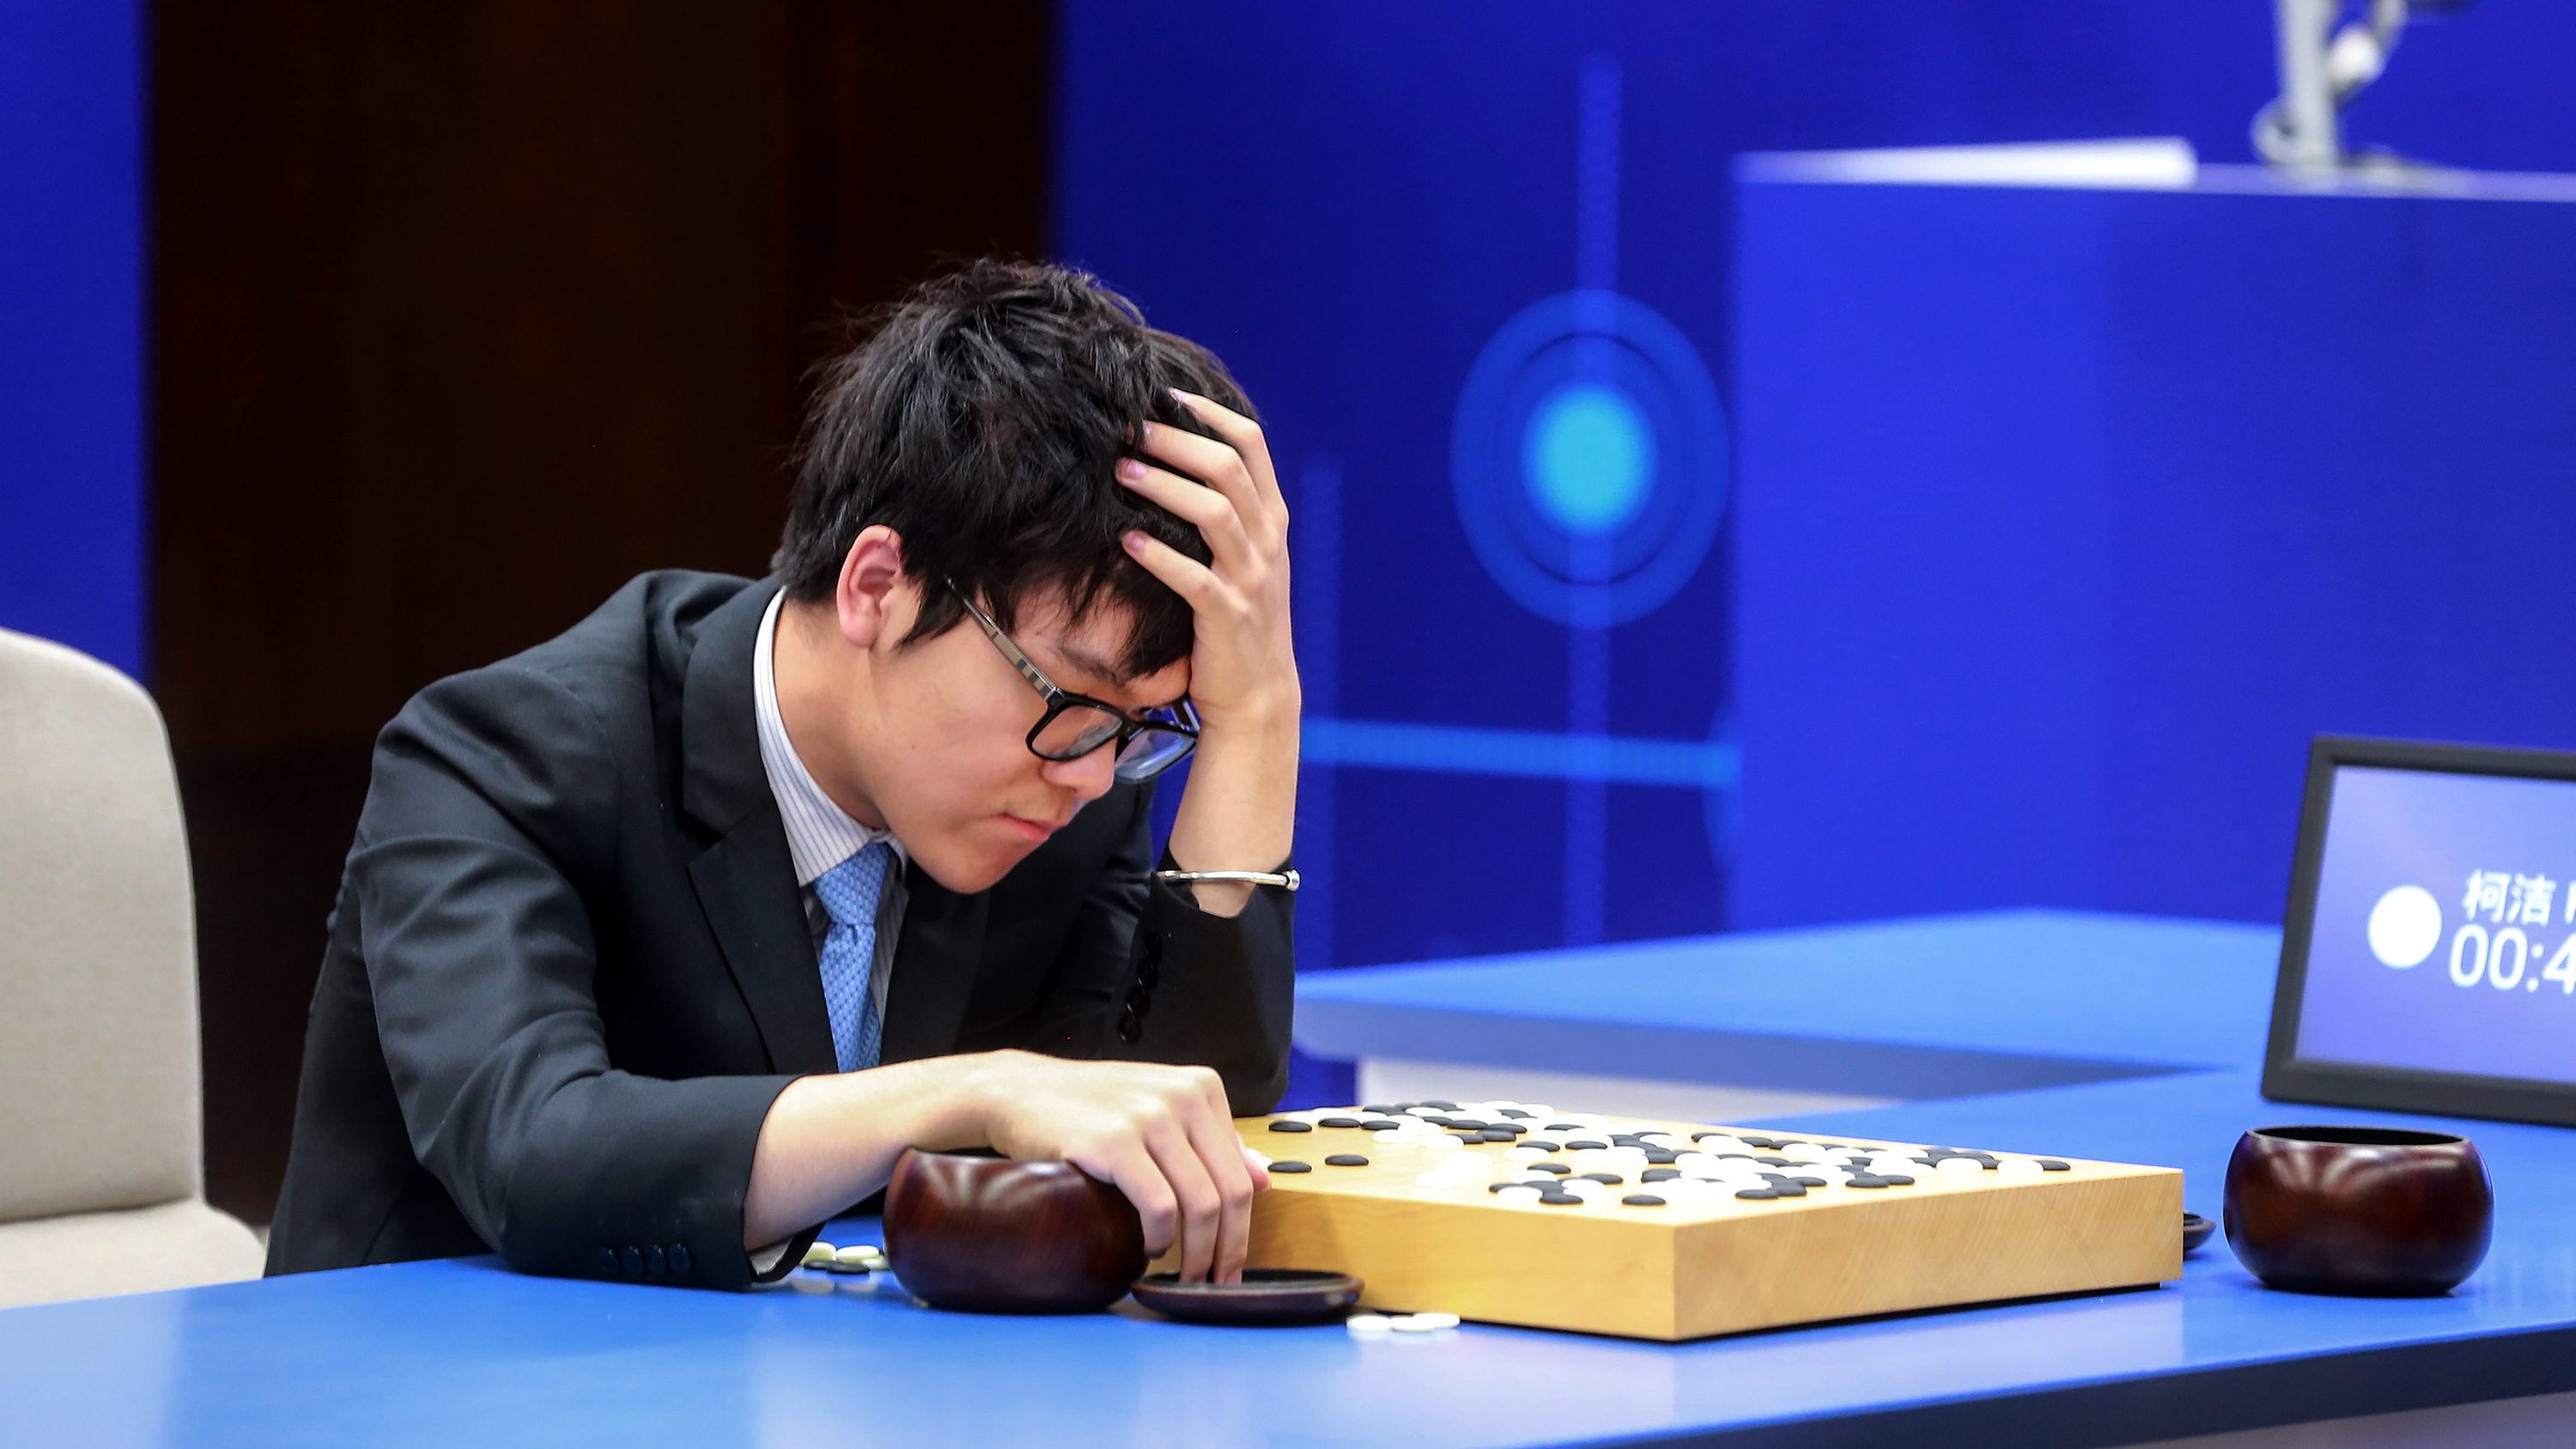
\includegraphics[scale=0.3]{images/alphago}
		\end{figure}
	``AlphaGo is the first computer program to defeat a professional human Go player, the first to defeat a Go world champion, and is arguably the strongest Go player in history." 
	
	More info: \href{https://www.deepmind.com/research/highlighted-research/alphago}{https://www.deepmind.com/research/highlighted-research/alphago}
	\end{frame}

	\begin{frame}
		\frametitle{Data}
		A \textbf{sample} (or example) is a collection of \textbf{attributes} (or features) that have been quantitatively measured from some object or event that we want the ML system to process.
		
		\vspace{5mm}
		
		
		A \textbf{dataset} is a collection of many samples.
		
		\begin{figure}
			\centering
			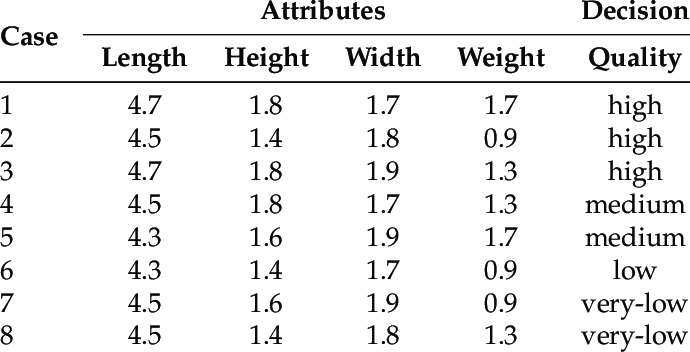
\includegraphics[scale=0.25]{images/data-example}
		\end{figure}
		
		
		We will deal with two types of attributes:
		
		
		\begin{itemize}
			\item Continuous = real numbers.
			\item Categorical (or discrete) = integers. 
		\end{itemize}
	\end{frame}

	\begin{frame}
		\frametitle{Data - Attributes}
		\begin{figure}
			\centering
			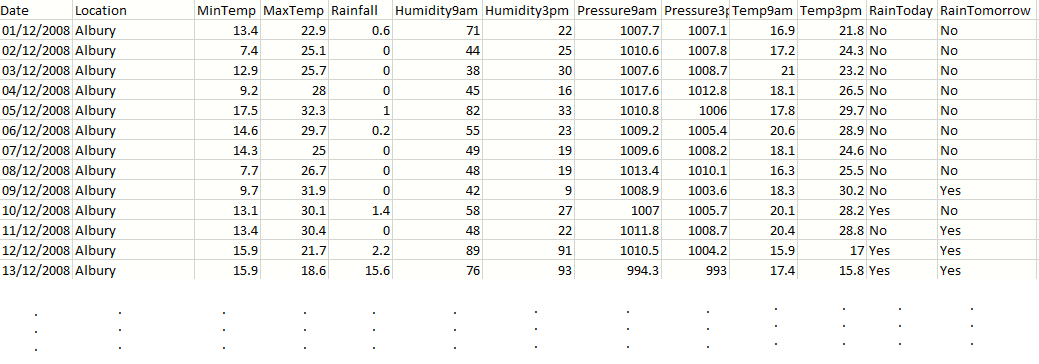
\includegraphics[scale=0.3]{images/data-attributes}
			\caption{``MinTemp" is an example of continuous attribute, while ``RainToday" is an example of categorical attribute (Yes = 1, No = 0).}
		\end{figure}
	\end{frame}

	\begin{frame}
		\frametitle{Data - Preprocessing}
		Preprocessing: preparing and manipulating the dataset to make it suitable for the model.
		\begin{itemize}
			\item \textbf{Data cleaning}. Identifying and correcting inconsistencies in the data.
			\item \textbf{Data transformation}. Converting the data into a suitable format
			\item \textbf{Data reduction}. Reducing the size of the dataset preserving as much as you can the important information
			\item \textbf{Data normalization}. Scaling the data to a common range (usually between 0 and 1 or -1 and 1).
		\end{itemize}
	\end{frame}
	

	\begin{frame}
		\frametitle{Tasks - Supervised learning}
		The \textbf{task} is the purpose of the application.
		
		\vspace{5mm}
		
		\textbf{Supervised learning} consists of tasks where each sample is associated with a \textbf{target} (also called label).
		
		%The term supervised learning originates from the view of the target being provided by an instructor or teacher who shows the ML system what to do.
		
	   	\begin{itemize}
			\item \textbf{Regression}. Predict a continuous dependent variable.
			
			Example: Predict the price of a house given its size.
			\item \textbf{Classification}.  Predict which categories/classes the input belongs to (categorical data).
			
			Example: Given an e-mail, predict if it is spam or not (\textsl{binary classification}).
		\end{itemize}
	\end{frame}

%	\begin{frame}
%		\frametitle{Supervised Learning - an example}
%		\begin{figure}
%			\centering
%			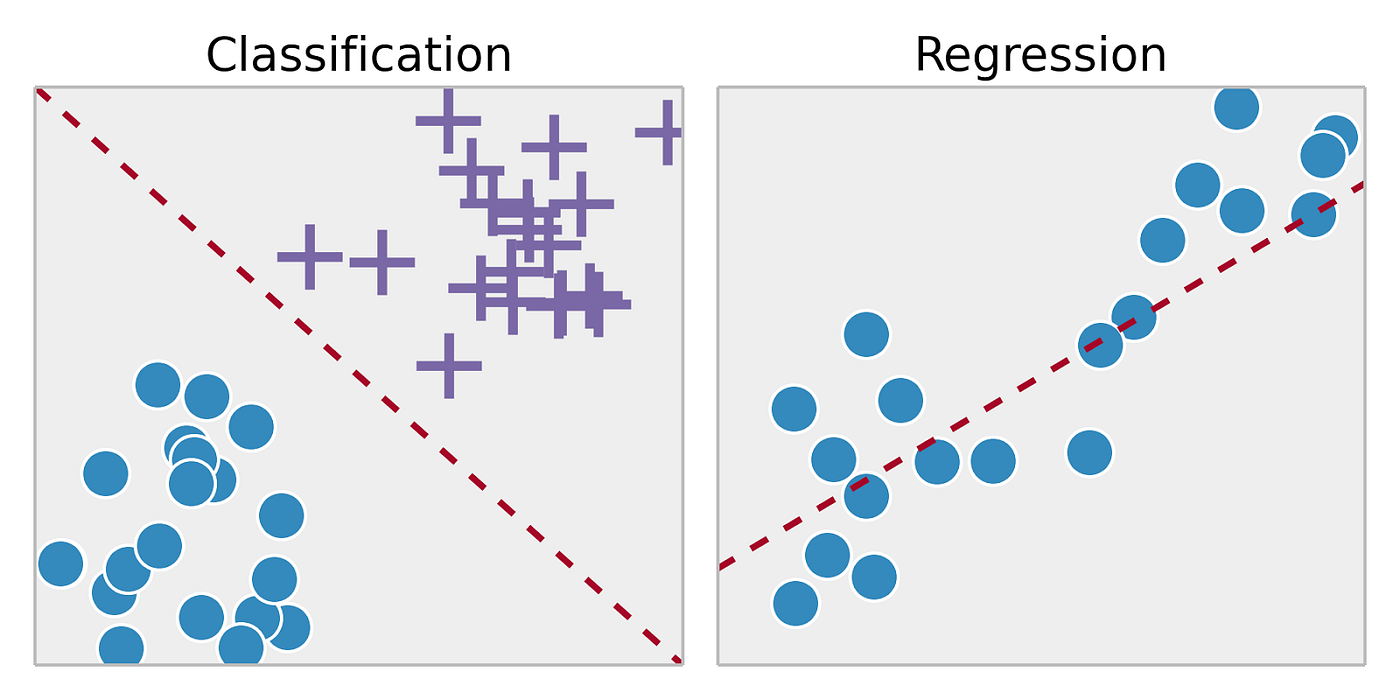
\includegraphics[scale=0.22]{images/supervised-learning}
%		\end{figure}
%	\end{frame}

	\begin{frame}
		\frametitle{Tasks- Unsupervised learning}
		\textbf{Unsupervised learning} tasks experience a dataset containing only features, but not a supervision signal (\textbf{unlabeled data}). %In other terms, we have to derive structure and different relationships from data.
		
		Examples:
		\begin{itemize}
			\item Take a collection of essays and find a way to automatically group them based on word frequency, sequence length, page counts etc.
			\item Recommender systems. Automatically provide suggestions for an item
			that is most pertinent to a particular user.
		\end{itemize} 
		
	\end{frame}

	\begin{frame}
		\frametitle{Unsupervised learning - an example}
		\begin{figure}
			\centering
			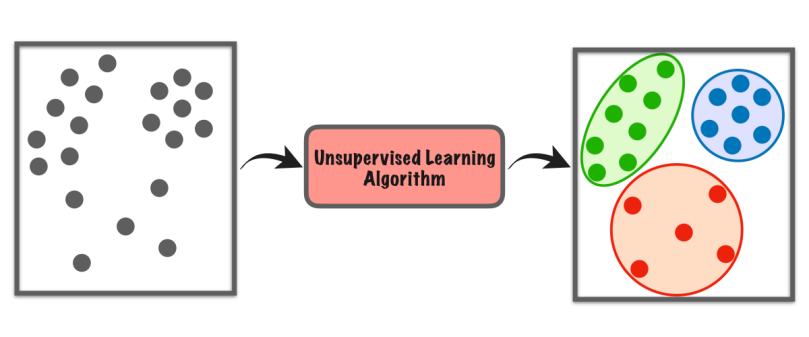
\includegraphics[scale=0.35]{images/unsupervised-learning}
			\caption{A clustering example.}
		\end{figure}
	\end{frame}

	\begin{frame}
		\frametitle{Model}
		
		A \textbf{model} is an abstract representation of a system using mathematical concepts. In the present context, the model operates on data to solve the task.
		
		\vspace{5mm}
		
		\textbf{Hypothesis}: a candidate model for the task.
		
		\textbf{Hypothesis space}: the class of models that the learning algorithm (see later) can produce.
		
		\vspace{5mm}
		
		\textbf{No free lunch theorem}: averaged over \textit{all} possible data-generating distributions, every classification algorithm has the same error rate when classifying previously unobserved points. However, we can design algorithms that perform well on specific kinds of probability distributions that we encounter in real-world applications.
		\end{frame}

	\begin{frame}
		\frametitle{Learning algorithm}
		A machine learning algorithm, in brief \textbf{learning algorithm}, is an algorithm that is able to learn from data.
		
		\vspace{5mm}
		
		To evaluate the abilities of a learning algorithm, we must design a quantitative measure of its performance. Usually this performance measure \textit{P} is specific to the task being carried out by the system.
		
		\vspace{5mm}
		
		The performance measure is called \textbf{cost function} (or \textsl{loss function}).
		
		\vspace{5mm}
		
		Example: a performance measure for the classification tasks is the \textbf{accuracy}. Accuracy is just the proportion of examples for which the model produces the correct output.
	\end{frame}

%	\begin{frame}
%		\frametitle{ML road map}
%		\begin{figure}
%			\centering
%			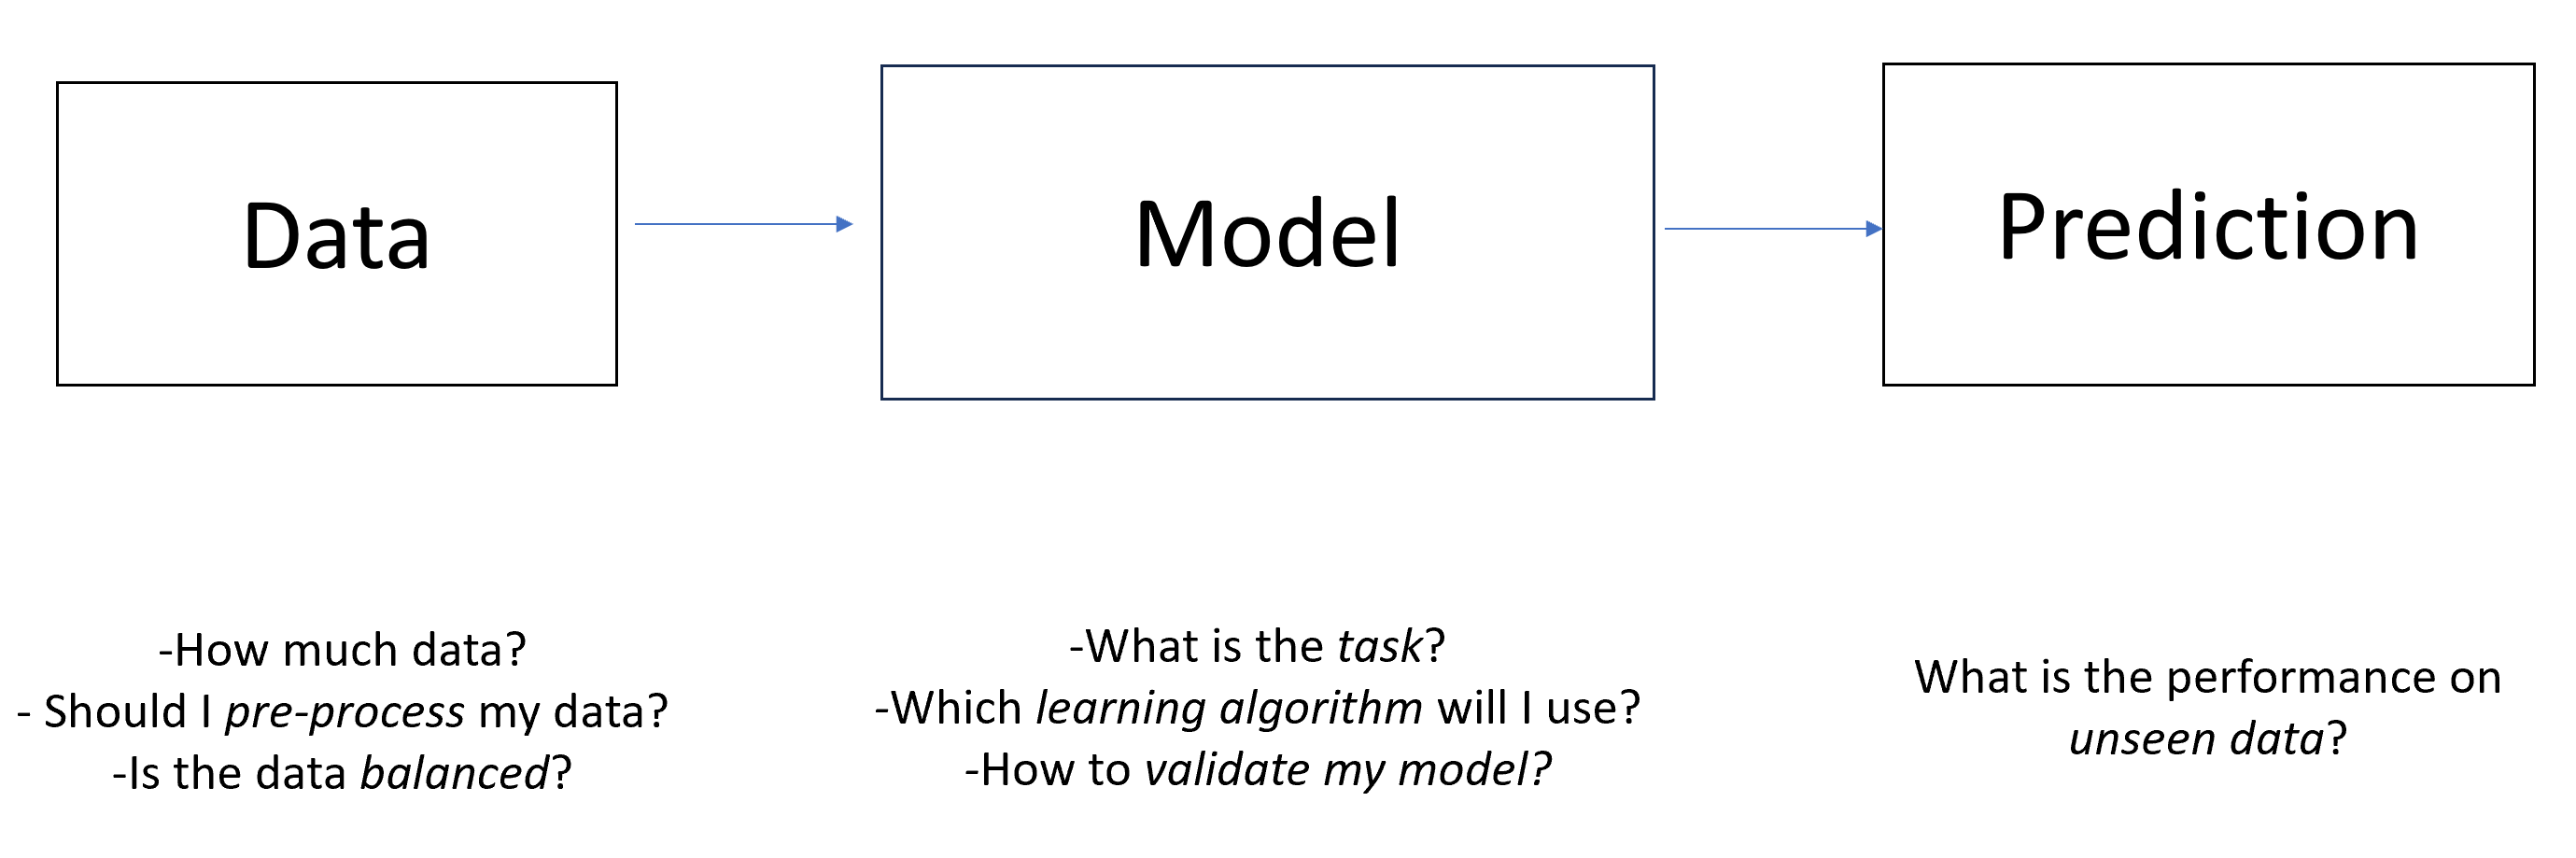
\includegraphics[scale=0.4]{images/road-map}
%		\end{figure}
%	\end{frame}

	
	
\end{document}